\documentclass{article}
\usepackage[utf8]{inputenc}
\usepackage{hyperref}
\usepackage{listings}
\usepackage{multimedia} % to embed movies in the PDF file
\usepackage{graphicx}
\usepackage{comment}
\usepackage[english]{babel}
\usepackage{amsmath}
\usepackage{amsfonts}
\usepackage{wrapfig}
\usepackage{multirow}
\usepackage{verbatim}
\usepackage{float}
\usepackage{cancel}
\usepackage{caption}
\usepackage{subcaption}
\usepackage{mathdots}
\usepackage{/home/cade/Homework/latex-defs}
\usepackage{/home/cade/Homework/jlcode}


\title{AMATH 586 Homework 5}
\author{Cade Ballew \#2120804}
\date{June 3, 2022}

\begin{document}
	
\maketitle
	
\section{Problem 1}
Consider the implicit upwind method for the advection equation $u_t + a u_x = 0$
\begin{align*}
	U_{j}^{n+1} = U_{j}^n  - \frac{ak}{h} \left( U_j^{n+1} - U_{j-1}^{n+1} \right).
\end{align*}
To derive the modified equation, we set $v(x,t)=U_j^n$ so that our scheme becomes
\[
\frac{v(x,t+k)-v(x,t)}{k}=-a\frac{v(x,t+k)-v(x-h,t+k)}{h}.
\]
Then, assuming that $v$ is sufficiently smooth,
\[
\text{LHS}=v_t+\frac{k}{2}v_{tt}+\OO(k^2).
\]
Also,
\begin{align*}
&\frac{v(x,t+k)-v(x-h,t+k)}{h}=v_x(x,t+k)-\frac{h}{2}v_{xx}(x,t+k)+\OO(h^2)\\&=
(v_x+kv_{xt}+\OO(k^2))-\frac{h}{2}(v_{xx}+\OO(k))+\OO(h^2)\\&=
v_x+kv_{xt}-\frac{h}{2}v_{xx}+\OO(h^2+hk+k^2).
\end{align*}
This yields that 
\begin{align*}
v_t=-av_x-\frac{k}{2}v_{tt}-akv_{xt}+\frac{ah}{2}v_{xx}+\OO(h^2+hk+k^2)=-av_x+\OO(h+k), 
\end{align*}
so we can substitute $v_{xt}=-av_{xx}$, $v_{tt}=a^2v_{xx}$ at the cost of a $\OO(h+k)$ term\footnote{Note that this then becomes higher order due to the scaling factors.}. Then,
\begin{align*}
v_t&=-av_x+\left(-\frac{a^2k}{2}+a^2k+\frac{ah}{2}\right)+\OO(h^2+hk+k^2)\\&=
-av_x+\left(\frac{a^2k}{2}+\frac{ah}{2}\right)+\OO(h^2+hk+k^2).
\end{align*}
Note that the modified equation for 
\begin{align*}
	U_{j}^{n+1} = U_{j}^n  - \frac{ak}{h} \left( U_j^{n} - U_{j-1}^{n} \right),
\end{align*}
derived in lecture is the same except that the coefficient on the $v_{xx}$ term is instead 
\[
\frac{ah}{2}-\frac{ak^2}{2},
\]
so our new PDE is instead well-posed when
\[
\frac{ak}{h}\geq-1
\]
if $a\geq0$.

\section{Problem 2}
Consider the method of lines discretization of the advection equation with a Dirichlet boundary conditions:
$$ \begin{cases} u_t + a u_{x} = 0, \quad a > 0,\\
	u(x,0) = \eta(x),\\
	u(0,t) = g_0(t), \end{cases} $$
given by
\begin{align*}
	U'(t) &= A U(t) + g(t),\\
	A &= \frac{-a}{2h} \begin{bmatrix} 0 & 1 \\
		-1 & 0 & 1 \\
		& -1 & \ddots & \ddots \\
		&& \ddots && 1\\
		&&& -1 & 0 \\
		&&1 & -4 & 3
	\end{bmatrix}, \quad g(t) = \begin{bmatrix} \frac{ak}{2h} g_0(t) \\ 0 \\ \vdots \\ 0 \end{bmatrix}.
\end{align*}
We perform von Neumann stability analysis on the scheme 
\begin{align*}
	U_j^{n+1} = \frac 1 2 ( U_{j-1}^{n-1} + U_{j+1}^{n-1}) - \frac{ak}{h} ( U_{j+1}^n - U_{j-1}^n).
\end{align*}
Namely, we take $U^n_j=s(\xi)^ne^{ij\xi h}$ which gives that 
\begin{align*}
s(\xi)^{n+1}e^{ij\xi h}=\frac{1}{2}s(\xi)^{n-1}\left(e^{i(j-1)\xi h}+e^{i(j+1)\xi h}\right)-\frac{ak}{h}s(\xi)^n\left(e^{i(j+1)\xi h}-e^{i(j-1)\xi h}\right),
\end{align*}
so
\begin{align*}
s(\xi)^2=\frac{1}{2}\left(e^{-i\xi h}+e^{i\xi h}\right)-\frac{ak}{h}s(\xi)\left(e^{i\xi h}-e^{-i\xi h}\right)=\cos(\xi h)-2i\frac{ak}{h}\sin(\xi h)s(\xi).
\end{align*}
Letting $\nu=\frac{ak}{h}$, we use the quadratic formula to solve this and get that 
\[
s(\xi)=-i\nu\sin(\xi h)\pm\sqrt{-\nu^2\sin^2(\xi h)+\cos(\xi h)}.
\] 
% Remember to do the rest of this problem lol
To see that $|s(\xi)| > 1$ for some $\xi$ regardless of $k,h$, consider $\xi^*=\frac{(2q+1)\pi}{h}$ for some $q\in\mathbb{Z}$. Then, $s(\xi^*)=\pm i$ and we choose the positive root. One can compute
\[
s'(\xi)=-ih\nu\cos(\xi h)\mp\frac{h\sin(\xi h)(2\nu^2\cos(\xi h)+1)}{2\sqrt{-\nu^2\sin^2(\xi h)+\cos(\xi h)}}
\]
which gives that $s'(\xi^*)=ih\nu$ which we note is normal to the unit circle at $i$. Continuity then implies that there exists some $\xi$ for which $s(\xi)$ has zero real part and imaginary part greater than 1, i.e., $|s(\xi)|>1$. \\
To derive the modified equation, we set $v(x,t)=U_j^n$ so that our scheme becomes 
\[
v(x,t+k)=\frac{1}{2}(v(x-h,t-k)+v(x+h,t-k))-\frac{ak}{h}(v(x+h,t)-v(x-h,t)).
\]
Taylor expanding,
\[
\text{LHS}=v+kv_t+\frac{k^2}{2}v_{tt}+\OO(k^3),
\]
\begin{align*}
&\frac{1}{2}(v(x-h,t-k)+v(x+h,t-k))=\frac{1}{2}(2v(x,t-k)+h^2v_{xx}(x,t-k)+\OO(h^4))\\&=
v(x,t-k)+\frac{h^2}{2}v_{xx}(x,t-k)+\OO(h^4)=\left(v-kv_t+\frac{k^2}{2}v_{tt}+\OO(k^3)\right)+\frac{h^2}{2}(v_{xx}+\OO(k))+\OO(h^4)\\&=
v-kv_t+\frac{k^2}{2}v_{tt}+\frac{h^2}{2}v_{xx}+\OO(h^4+h^2k+k^3),
\end{align*}
\begin{align*}
&\frac{ak}{h}(v(x+h,t)-v(x-h,t))=\frac{ak}{h}\left(2hv_x+O(h^3)\right)=2akv_x+\OO(kh^2),
\end{align*}
so 
\[
\text{RHS}=v-2akv_x+\frac{h^2}{2}v_{xx}-kv_t+\frac{k^2}{2}v_{tt}+\OO(h^4+h^2k+k^3).
\]
Equating these,
\begin{align*}
	v_t=-av_x+\frac{h^2}{4k}v_{xx}+\OO\left(\frac{h^4}{k}+h^2+k^2\right).
\end{align*}
%so we can write that 
%\begin{align*}
%v_t=-av_x+\left(\frac{h^2}{4k}+\frac{a^2k}{4}\right)v_{xx}+\OO\left(\frac{h^4}{k}+h^2+k^2\right).
%\end{align*}
If we choose $k\approx ch^2$, then our equation becomes
\[
v_t\approx-av_x+\frac{1}{4c}v_{xx}+\OO(h^2)
\]
which always has a nonnegative diffusion constant meaning that the PDE is well-posed; however, we actually lose consistency because the $v_{xx}$ term does not vanish as $k,h\to\infty$, meaning that this choice is not reasonable as then the modified equations don't correspond to the correct PDE.
\section{Problem 3}
Consider the wave equation with periodic boundary conditions on $[0,1]$
\begin{align*}
	\begin{cases}
		u_{tt} = c^2 u_{xx}, \quad c > 0,\\
		u(x,0) = f(x),\\
		u_t(x,0) = g(x),\\
		u(0,t) = u(1,t),\\
		u_x(0,t) = u_x(1,t).
	\end{cases}
\end{align*}
with $f(x) = \exp( -20(x-1/2)^2 )$, $g(x) = \sin(4\pi x)$, $c = 1$. To solve this numerically, we note that 
\[
(\partial_t-c\partial_x)(\partial_t+c\partial_x)u=0,
\]
so we define $w=(\partial_t-c\partial_x)u$ so that the system 
\[
\begin{pmatrix}
u\\w
\end{pmatrix}_t+c\begin{pmatrix}
-1 &0\\0&1
\end{pmatrix}\begin{pmatrix}
u\\w
\end{pmatrix}_x=\begin{pmatrix}
w\\0
\end{pmatrix}
\]
holds. Note that 
\[
w(x,0)=u_t(x,0)-cu_x(x,0)=g(x)-cf'(x)
\]
and 
\[
w(0,t)=u_t(0,t)-cu_x(0,t)=u_t(1,t)-cu_x(1,t)=w(1,t),
\]
so $w$ is also periodic and its initial condition can be computed directly. Note that in the our system, $w$ depends only on itself so we may solve this system numerically as two separate equations at each iteration. Namely, we solve 
\[
u_t-cu_x=w
\]
then
\[
w_t+cw_x=0.
\]
We do this, we essentially apply Lax-Wendroff to each problem under the framework of the advection equation with periodic boundary conditions albeit slightly modified for the first problem. The centered difference MOL discretization gives that
\[
\begin{pmatrix}
\\	u'_j(t) \\ \\
\end{pmatrix}-\frac{c}{2h}S\begin{pmatrix}
\\	u_j(t) \\ \\
\end{pmatrix}=\begin{pmatrix}
\\	w_j(t) \\ \\
\end{pmatrix}
\] 
where 
\begin{align*}
	S = \begin{pmatrix}
		0  & 1 &&&& -1\\
		-1 & 0 & 1 \\
		& -1 & 0 & 1 & \\
		&&\ddots & \ddots & \ddots \\
		&&&-1 & 0 & 1 \\
		1 &&&& -1 & 0 \end{pmatrix}.
\end{align*}
Applying the modified second order Taylor method to this problem then gives that
\[
\begin{pmatrix}
	\\	u^{n+1}_j \\ \\
\end{pmatrix}=\begin{pmatrix}
\\	u^n_j \\ \\
\end{pmatrix}+\frac{ck}{2h}S\begin{pmatrix}
\\	u^n_j \\ \\
\end{pmatrix}-\frac{c^2k^2}{2h^2}A\begin{pmatrix}
\\	u^n_j \\ \\
\end{pmatrix}+k\begin{pmatrix}
	\\	w_j^n \\ \\
\end{pmatrix}
\] 
where 
\begin{align*}
	A = \begin{pmatrix}
		2  & -1 &&&& -1\\
		-1 & 2 & -1 \\
		& -1 & 2 & -1 & \\
		&&\ddots & \ddots & \ddots \\
		&&&-1 & 2 & -1 \\
		-1 &&&& -1 & 2 \end{pmatrix}.
\end{align*}
Note that this is just Lax-Wendroff with the advection coefficient negated and $w$ introduced as a forcing term. Since we will compute $w_j^n$ using vanilla Lax-Wendroff, that term will be second order accurate meaning that our entire approximation for $u$ will be second order accurate. In that vein, we will compute $w$ at each step by
\[
\begin{pmatrix}
	\\	w^{n+1}_j \\ \\
\end{pmatrix}=\begin{pmatrix}
	\\	w^n_j \\ \\
\end{pmatrix}-\frac{ck}{2h}S\begin{pmatrix}
	\\	w^n_j \\ \\
\end{pmatrix}-\frac{c^2k^2}{2h^2}A\begin{pmatrix}
	\\	w^n_j \\ \\
\end{pmatrix}.
\] 
Since we are using Lax-Wendroff, it is known to be stable when 
\[
\frac{|c|k}{h}\leq1.
\]
To solve this problem numerically, we take $h=0.01$, so we choose $k=h$ to meet the stability criterion. Solving until $t=3$, we produce the following plots.
\begin{figure}[H]
	\centering
	\begin{subfigure}{0.495\linewidth}
		\centering
		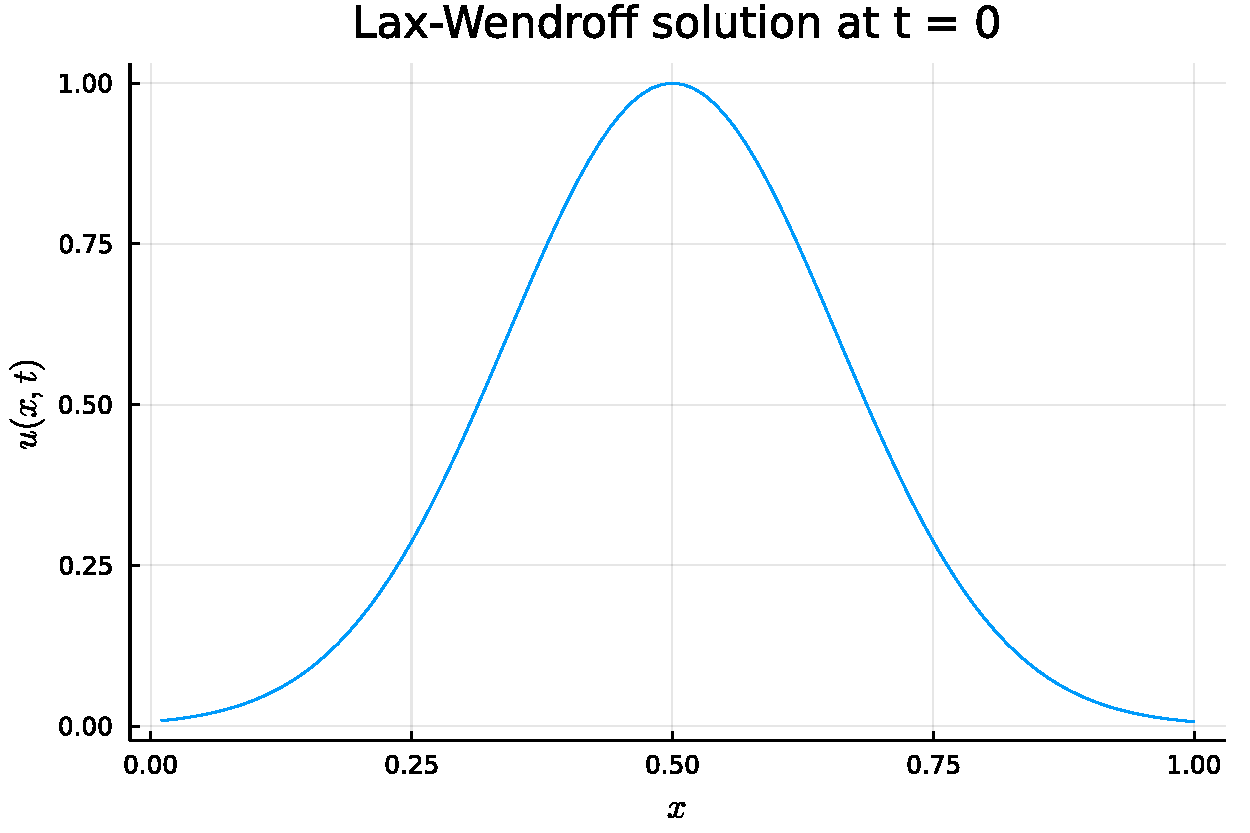
\includegraphics[width=\linewidth]{p3t0.pdf}
	\end{subfigure}
	\begin{subfigure}{0.495\linewidth}
		\centering
		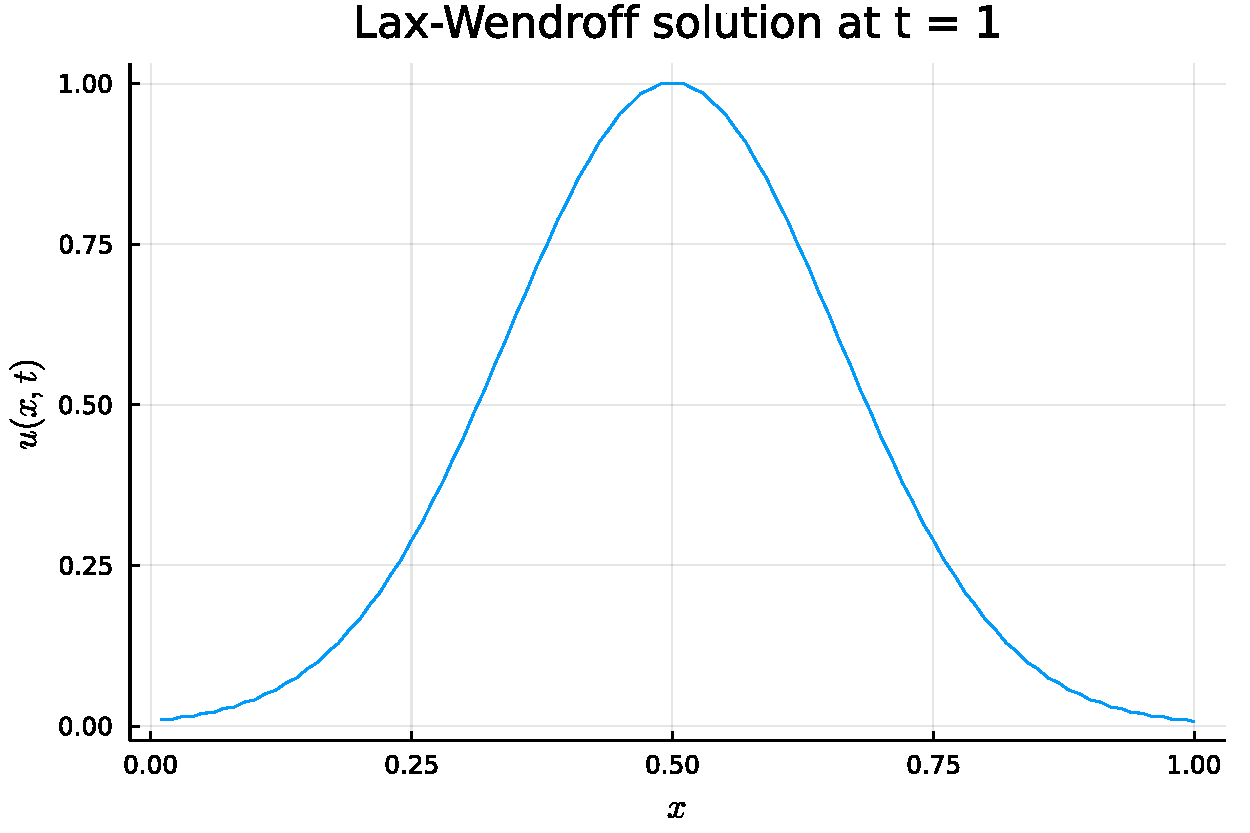
\includegraphics[width=\linewidth]{p3t1.pdf}
	\end{subfigure}
	\begin{subfigure}{0.495\linewidth}
		\centering
		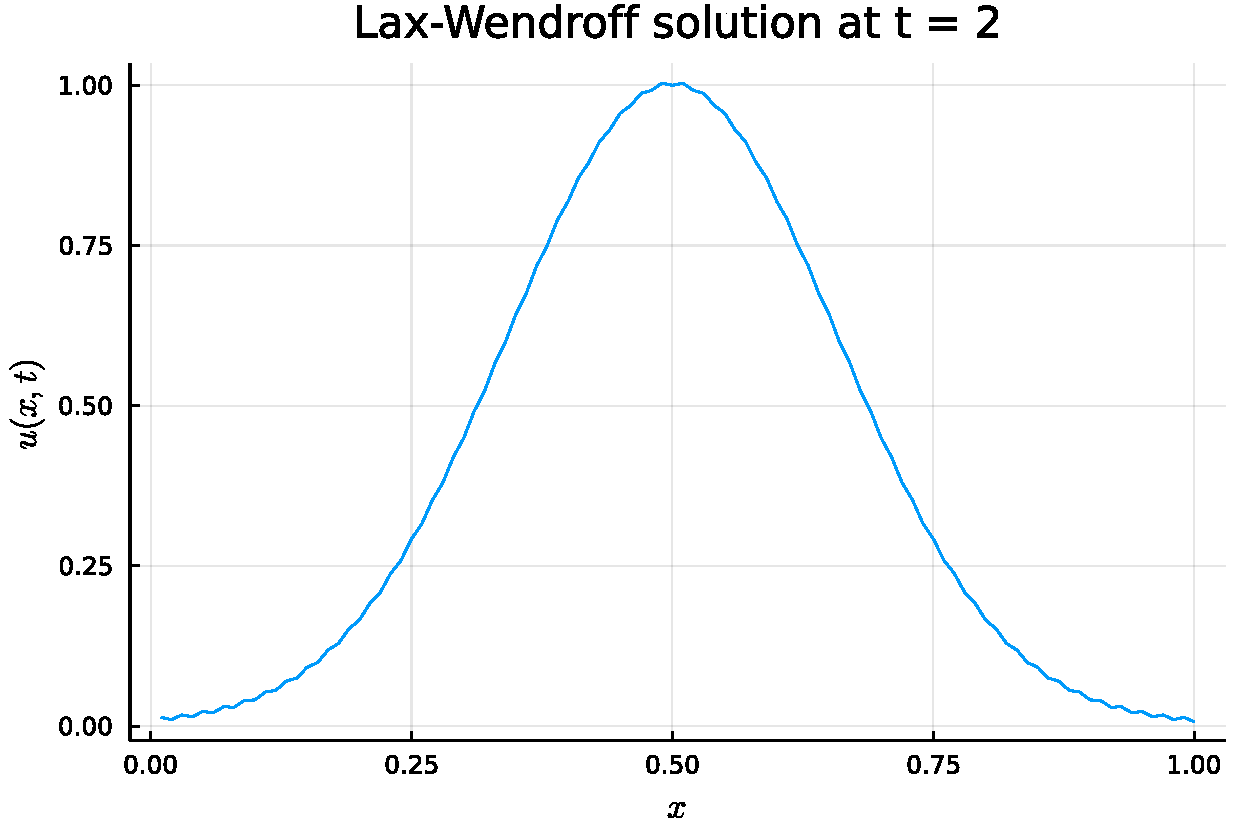
\includegraphics[width=\linewidth]{p3t2.pdf}
	\end{subfigure}
	\begin{subfigure}{0.495\linewidth}
		\centering
		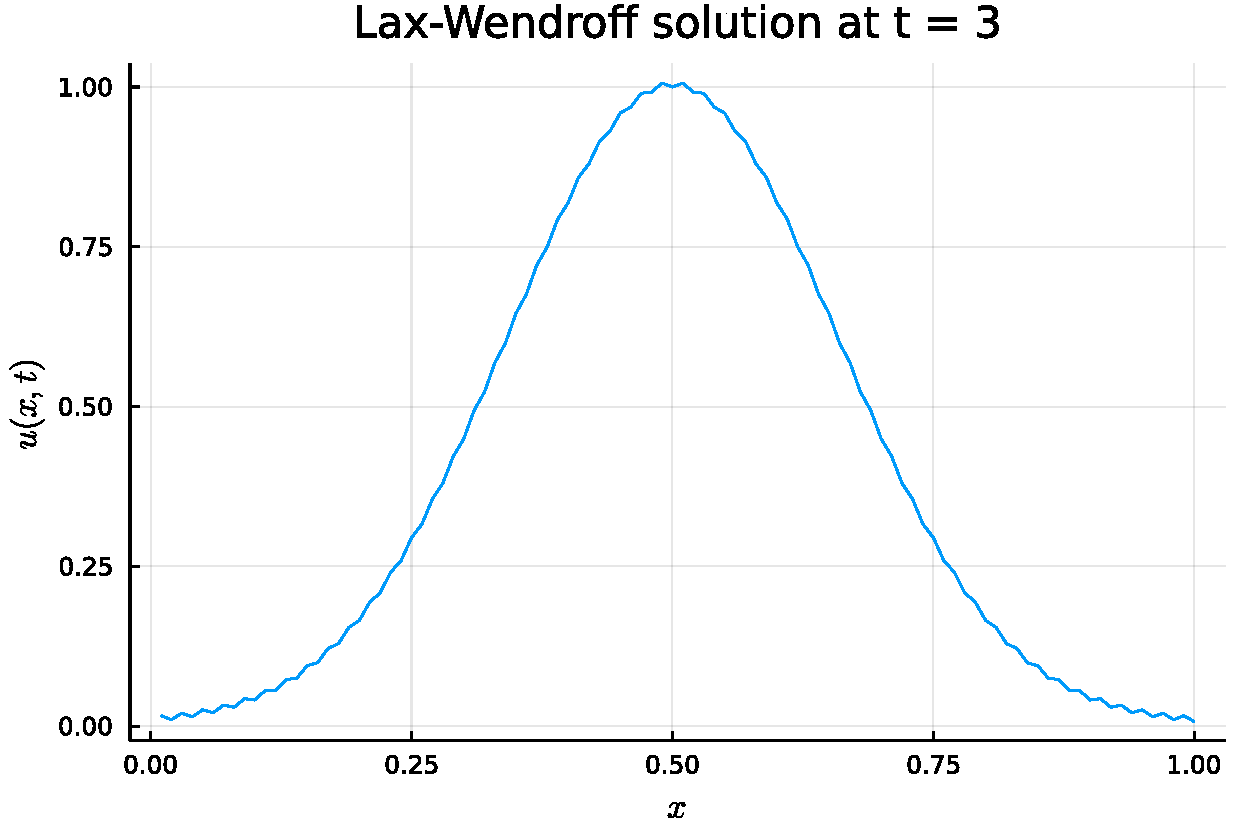
\includegraphics[width=\linewidth]{p3t3.pdf}
	\end{subfigure}
\end{figure}
Note that while these plots are nearly identical, $u$ does in fact change at each timestep and just makes it back to this at each integral time.\\
See Appendix A for the Julia code used to solve this. 

\section{Problem 4}
Consider the non-constant coefficient reaction diffusion equation
\begin{align*}
	\begin{cases}
		u_t = \kappa(x) u_{xx} + u(1-u)(u-1/2), \quad \kappa(x) = \sin^4(2\pi x - \pi),\\
		u(x,0) = \eta(x),\\
		u(0,t) = u(1,t),\\
		u_x(0,t) = u_x(1,t).
	\end{cases}
\end{align*}
with initial condition
\begin{align*}
	\eta(x) = \frac{ ( 1 + \mathrm{tanh}(20(x-0.25)) ) ( 1 + \mathrm{tanh}(20(-x+0.75)))}{4}.
\end{align*}
We solve this problem by forming the diffusion matrix
\begin{align*}
	A_{\kappa} = \frac{1}{h^2} \mathrm{diag}(\kappa(x_1),\ldots,\kappa(x_m)) A, \quad A  = \begin{bmatrix}
		-2  & 1 &&& 1\\
		1 & -2 & 1 \\
		& 1 & -2 & 1\\
		&& \ddots & \ddots & \ddots \\
		1&&& 1 & -2 \end{bmatrix}.
\end{align*}
Using Julia, we write a function {\tt CN(U,k)} that performs a step of size $k$ for trapezoid applied to the MOL discretization $U'(t) = A_{\kappa} U(t)$ and then use RK2 (5.30) to write a function {\tt RK2(U,k)} performs one time step of $U'(t) = U(t)(1-U(t))(U(t) - 1/2)$ with time step $k$. Finally, we solve the problem to $t=1$ using the Strang splitting scheme 
\begin{verbatim}
	U = RK2(U,k/2)
	U = CN(U,k)
	U = RK2(U,k/2)
\end{verbatim}
Doing this produces the following plots at various timesteps.
\begin{figure}[H]
	\centering
	\begin{subfigure}{0.495\linewidth}
		\centering
		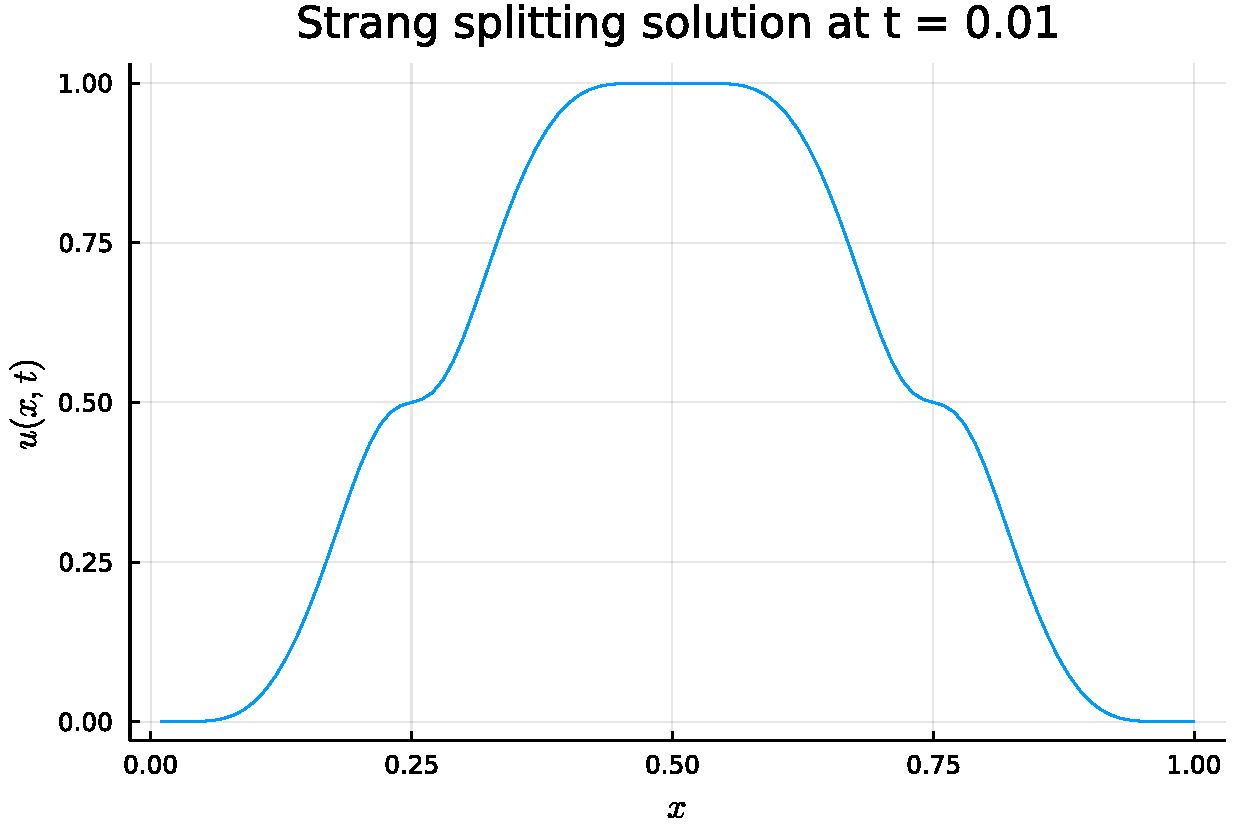
\includegraphics[width=\linewidth]{p4at0.01.pdf}
	\end{subfigure}
	\begin{subfigure}{0.495\linewidth}
		\centering
		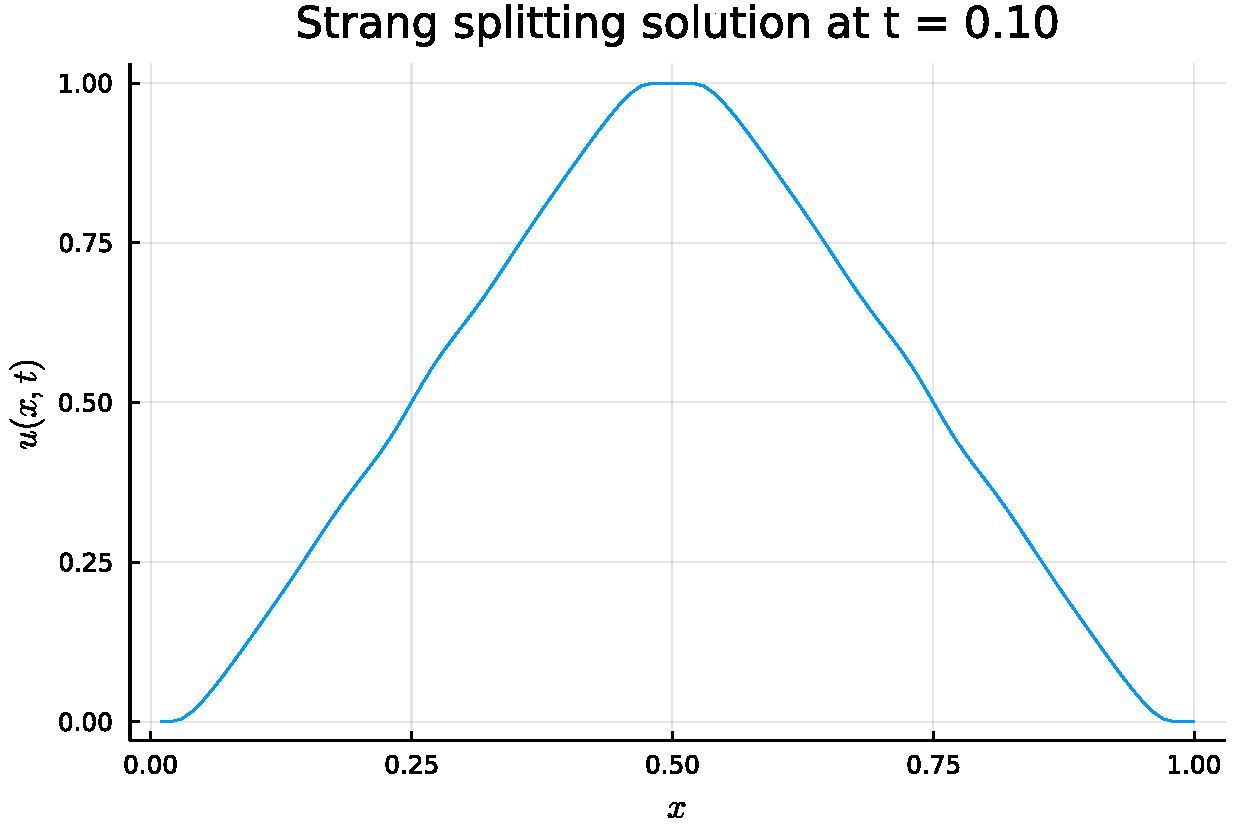
\includegraphics[width=\linewidth]{p4at0.10.pdf}
	\end{subfigure}
	\begin{subfigure}{0.495\linewidth}
		\centering
		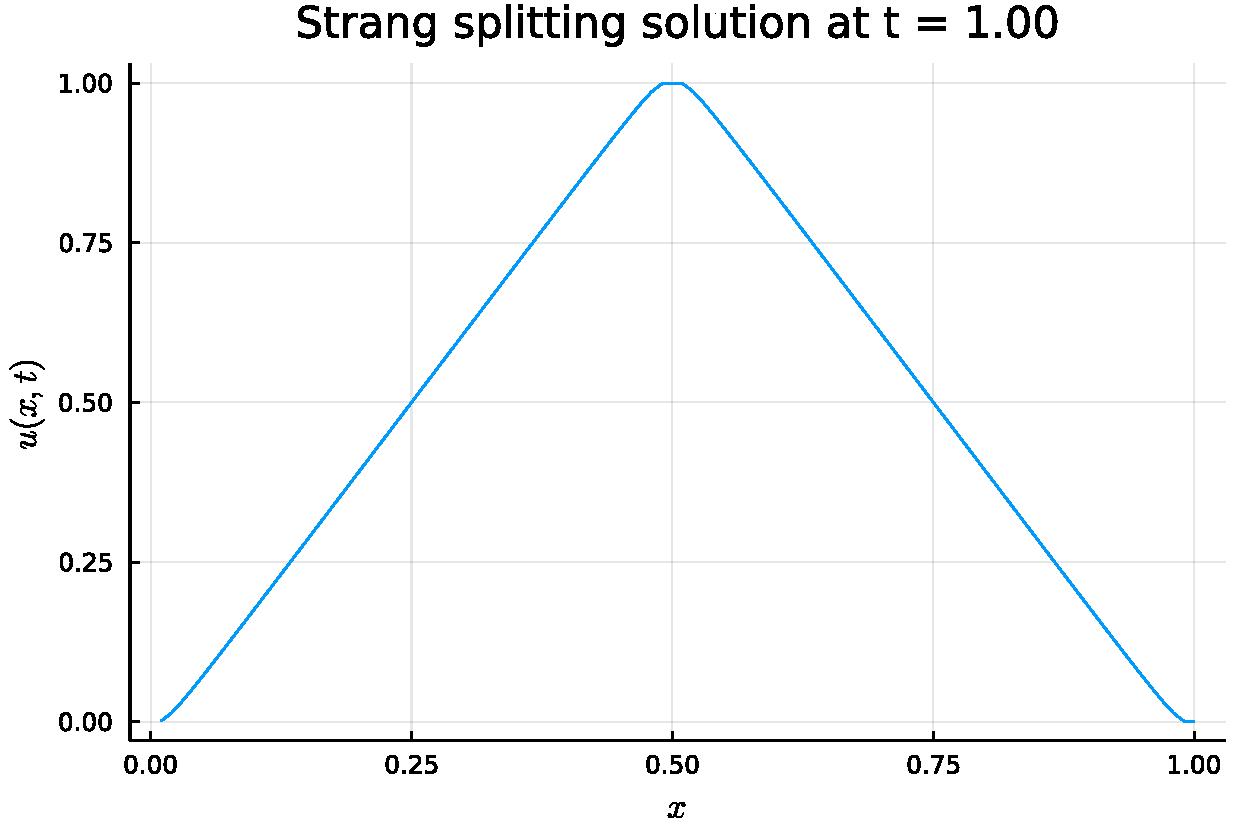
\includegraphics[width=\linewidth]{p4at1.00.pdf}
	\end{subfigure}
\end{figure}
If we instead take $\kappa(x) = \cos^4(2\pi x)$, we observe the following plots.
\begin{figure}[H]
	\centering
	\begin{subfigure}{0.495\linewidth}
		\centering
		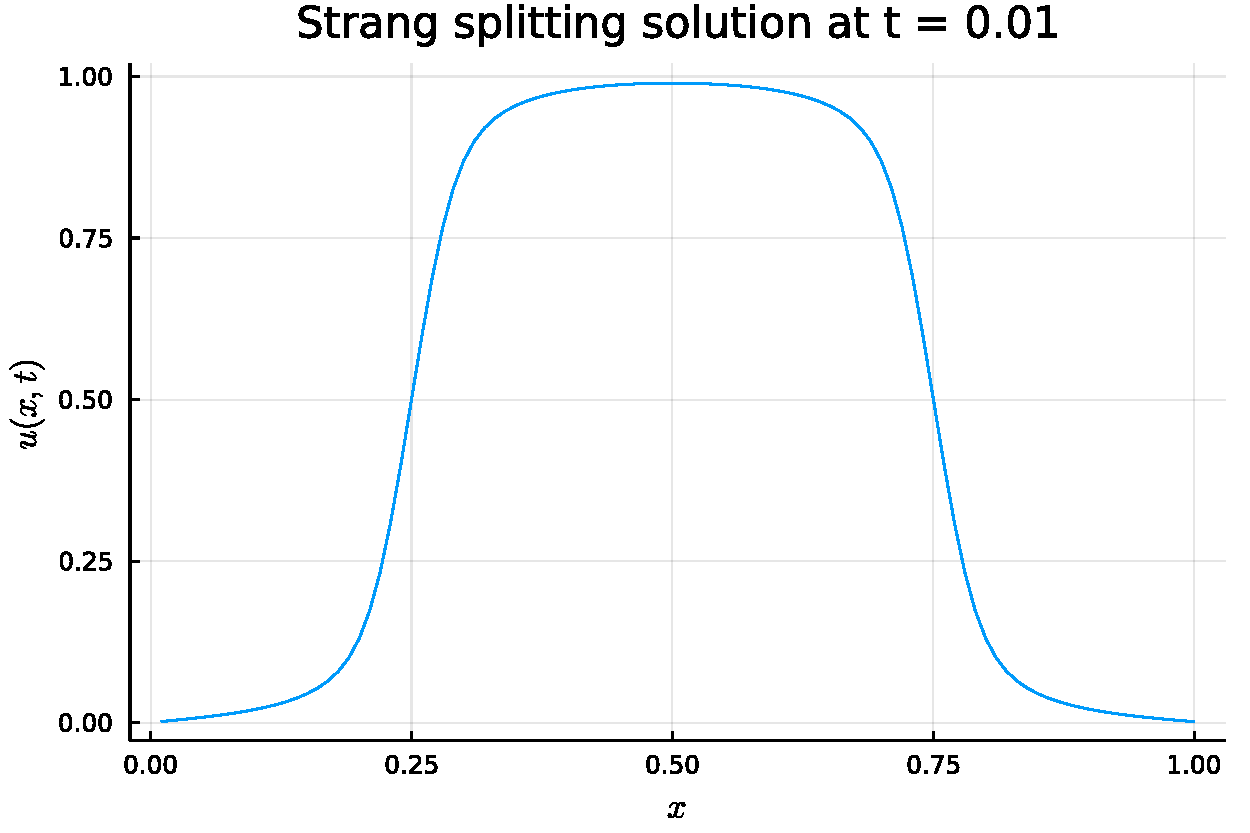
\includegraphics[width=\linewidth]{p4bt0.01.pdf}
	\end{subfigure}
	\begin{subfigure}{0.495\linewidth}
		\centering
		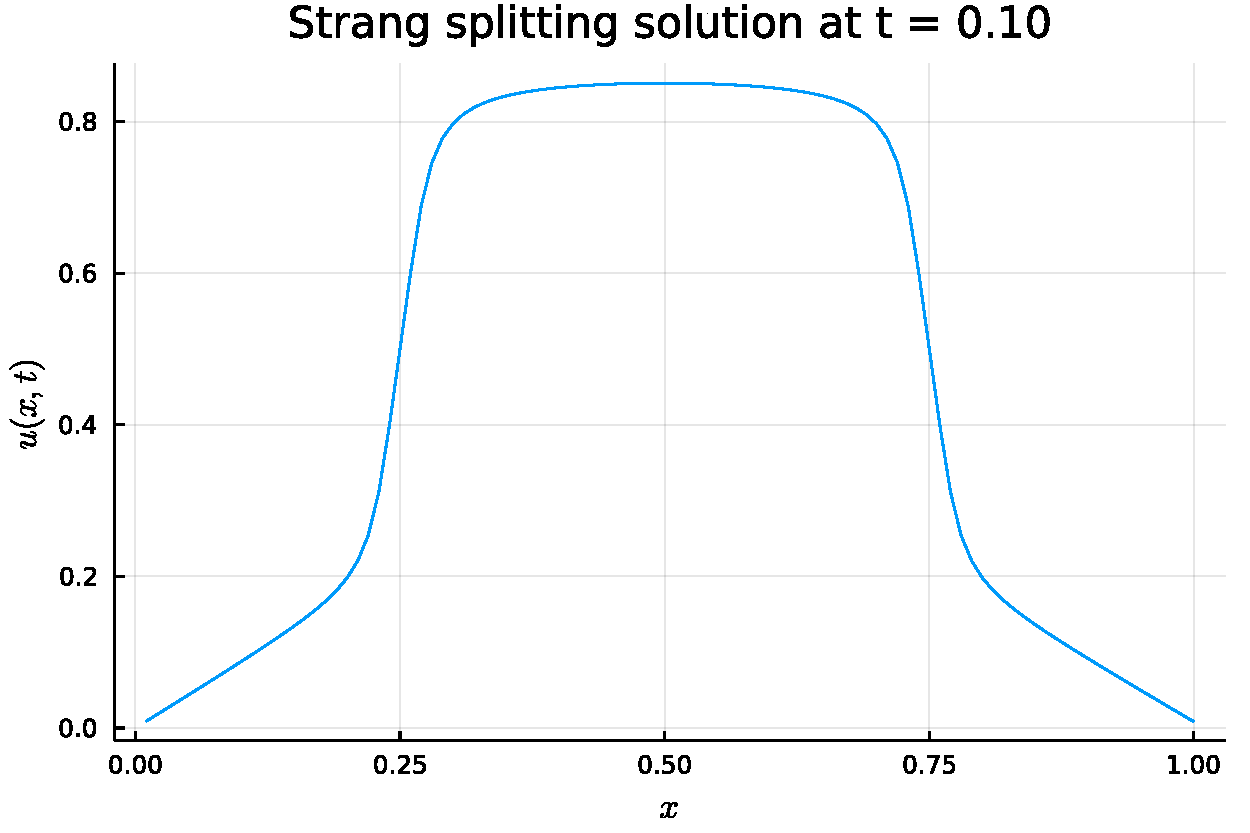
\includegraphics[width=\linewidth]{p4bt0.10.pdf}
	\end{subfigure}
	\begin{subfigure}{0.495\linewidth}
		\centering
		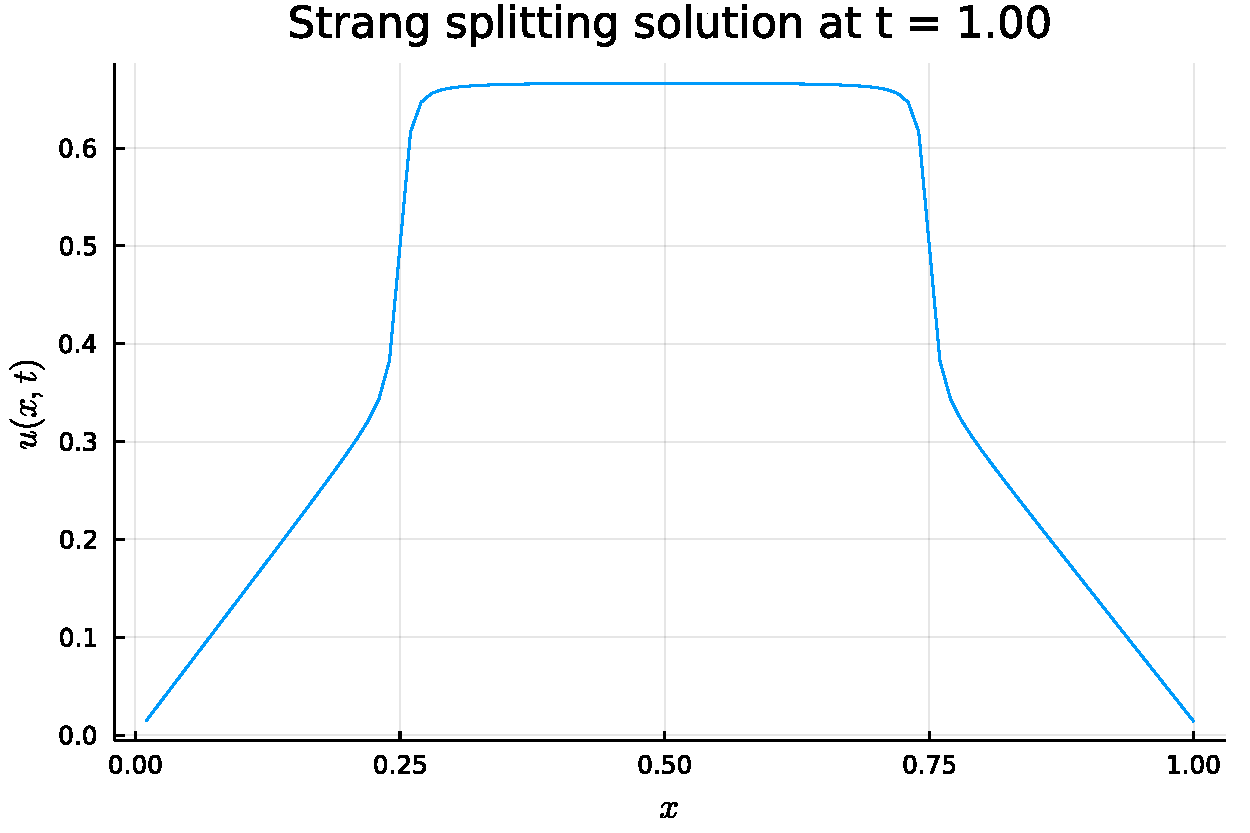
\includegraphics[width=\linewidth]{p4bt1.00.pdf}
	\end{subfigure}
\end{figure}
See Appendix A for the Julia code used to solve this problem. 

\section{Problem 5}
Consider two $n \times n$ matrices $A$, $B$. Then, by definition, 
\begin{align*}
e^{k(A+B)}&=I+k(A+B)+\frac{k^2}{2}(A+B)^2+\OO(k^3)\\&=
I+k(A+B)+\frac{k^2}{2}(A^2+AB+BA+B^2)+\OO(k^3)
\end{align*}
and 
\begin{align*}
&e^{k/2 A}e^{k B}e^{k/2 A}\\&=
\left(I+\frac{k}{2}A+\frac{(k/2)^2}{2}A^2+\OO(k^3)\right)\left(I+kB+\frac{k^2}{2}B^2+\OO(k^3)\right)\left(I+\frac{k}{2}A+\frac{(k/2)^2}{2}A^2+\OO(k^3)\right)\\&=
\left(I+k\left(\frac{1}{2}A+B\right)+k^2\left(\frac{1}{2}AB+\frac{1}{8}A^2+\frac{1}{2}B^2\right)+\OO(k^3)\right)\left(I+\frac{k}{2}A+\frac{(k/2)^2}{2}A^2+\OO(k^3)\right)\\&=
I+k\left(\frac{1}{2}A+B+\frac{1}{2}A\right)+k^2\left(\left(\frac{1}{2}A+B\right)\frac{1}{2}A+\left(\frac{1}{2}AB+\frac{1}{8}A^2+\frac{1}{2}B^2\right)+\frac{1}{8}A^2\right)+\OO(k^3)\\&=
I+k(A+B)+k^2\left(\frac{1}{2}A^2+\frac{1}{2}BA+\frac{1}{2}AB+\frac{1}{2}B^2\right)+\OO(k^3)\\&=
I+k(A+B)+\frac{k^2}{2}(A^2+AB+BA+B^2)+\OO(k^3).
\end{align*}
Thus,
\[
e^{k(A+B)} - e^{k/2 A}e^{k B}e^{k/2 A} = O(k^3).
\]

\section{Problem 6}
Consider the Jacobi iteration (4.4) for the linear system $A u=f$ arising from a centered difference approximation of the boundary value problem $u_{x x}(x)=f(x)$ which is given by
\[
u_j^{n+1}=\frac{1}{2}(u^n_{j-1}+u_{j+1}^n-h^2f_j).
\]
Consider the heat equation $u_{t}(x, t)=u_{x x}(x, t)-f(x)$. Applying the centered difference discretization, the MOL equations are then given by
\[
u_j'(t)=\frac{u_{j+1}(t)-2u_j(t)+u_{j-1}(t)}{h^2}-f_j.
\] 
Applying forward Euler to this system, we then have that 
\[
\frac{u_j^{n+1}-u_j^n}{k}=\frac{u_{j+1}^n-2u_j^n+u_{j-1}^n}{h^2}-f_j.
\]
Then, letting $k=h^2/2$, we find that 
\begin{align*}
u_j^{n+1}&=u_j^n+k\left(\frac{u_{j+1}^n-2u_j^n+u_{j-1}^n}{h^2}-f_j\right)=u_j^n+\frac{h^2}{2}\frac{u_{j+1}^n-2u_j^n+u_{j-1}^n}{h^2}-\frac{h^2}{2}f_j\\&=
u_j^n+\frac{1}{2}(u_{j+1}^n-2u_j^n+u_{j-1}^n-h^2f_j)=\frac{1}{2}(u_{j+1}^n+u_{j-1}^n-h^2f_j).
\end{align*}
Thus, the Jacobi iteration can be interpreted as forward Euler time stepping applied to the MOL equations arising from a centered difference discretization of the heat equation $u_{t}(x, t)=u_{x x}(x, t)-f(x)$ with time step $k=\frac{1}{2} h^{2}$.

\section{Problem 7}
Now, consider the Gauss-Seidel method for solving the linear system
$$
U_{j}^{n+1}=\frac{1}{2}\left(U_{j-1}^{n+1}+U_{j+1}^{n}-h^{2} f\left(x_{j}\right)\right).
$$
Considering this as a finite difference equation, we derive the modified equation by letting $U^n_j=v(x,t)$. Then, the scheme can be written as
\[
2v(x,t+k)=v(x-h,t+k)+v(x+h,t)-h^2f(x).
\]
Taylor expanding, 
\[
\text{LHS}=2v+2kv_t+k^2v_{tt}+\OO(k^3)
\]
and 
\begin{align*}
\text{RHS}&=v(x,t+k)-hv_x(x,t+k)+\frac{h^2}{2}v_{xx}(x,t+k)+\OO(h^3)+v+hv_x+\frac{h^2}{2}v_{xx}-h^2f(x)\\&=
(v+kv_t+k^2v_{tt}+\OO(k^3))-h(\cancel{v_x}+kv_{xt}+\OO(k^2))+\frac{h^2}{2}(v_{xx}+\OO(k))+\OO(h^3)\\&+v+\cancel{hv_x}+\frac{h^2}{2}v_{xx}-h^2f(x)\\&=
2v+h^2v_{xx}+kv_t+k^2v_{tt}-khv_{xt}+\OO(h^3+k^2h+h^2k+k^3).
\end{align*}
Then, we find that our modified equation is given by
\[
v_t=\frac{h^2}{k}v_{xx}-hv_{xt}-\frac{h^2}{k}f(x)+\frac{1}{k}\OO(h^3+k^2h+h^2k+k^3).
\]
Letting $k=h^2/2$, we then find that 
\begin{align*}
v_t=2v_{xx}-hv_{xt}-2f(x)+\OO(h)=2(v_{xx}-f(x))+\OO(h).
\end{align*}
This implies that Gauss-Seidel is consistent with the PDE $u_t(x,t)=2(u_{xx}(x,t)-f(x))$ which of course is twice the RHS of the PDE from problem 6. This relates to the observation in Section 4.2.1 that Gauss-Seidel takes roughly half as many iterations as Jacobi to converge as each timestep of the PDE corresponding to Gauss-Siedel then moves twice as far compared to those of the PDE corresponding to Jacobi.

\section{Appendix A}
The following Julia code is used for Problem 3.
\jlinputlisting{Problem3.jl}
The following Julia code is used for Problem 4.
\jlinputlisting{Problem4.jl}

\end{document}
